\section{Antecedentes}

\begin{frame}
	\frametitle{Desalinizador autónomo}
	En 2018 se desarrolló un destilador solar activo e híbrido, capaz de destilar hasta \SI{10}{\litre} por día en días soleados usando precalentamiento de agua\\
	\begin{figure}
		\centering
		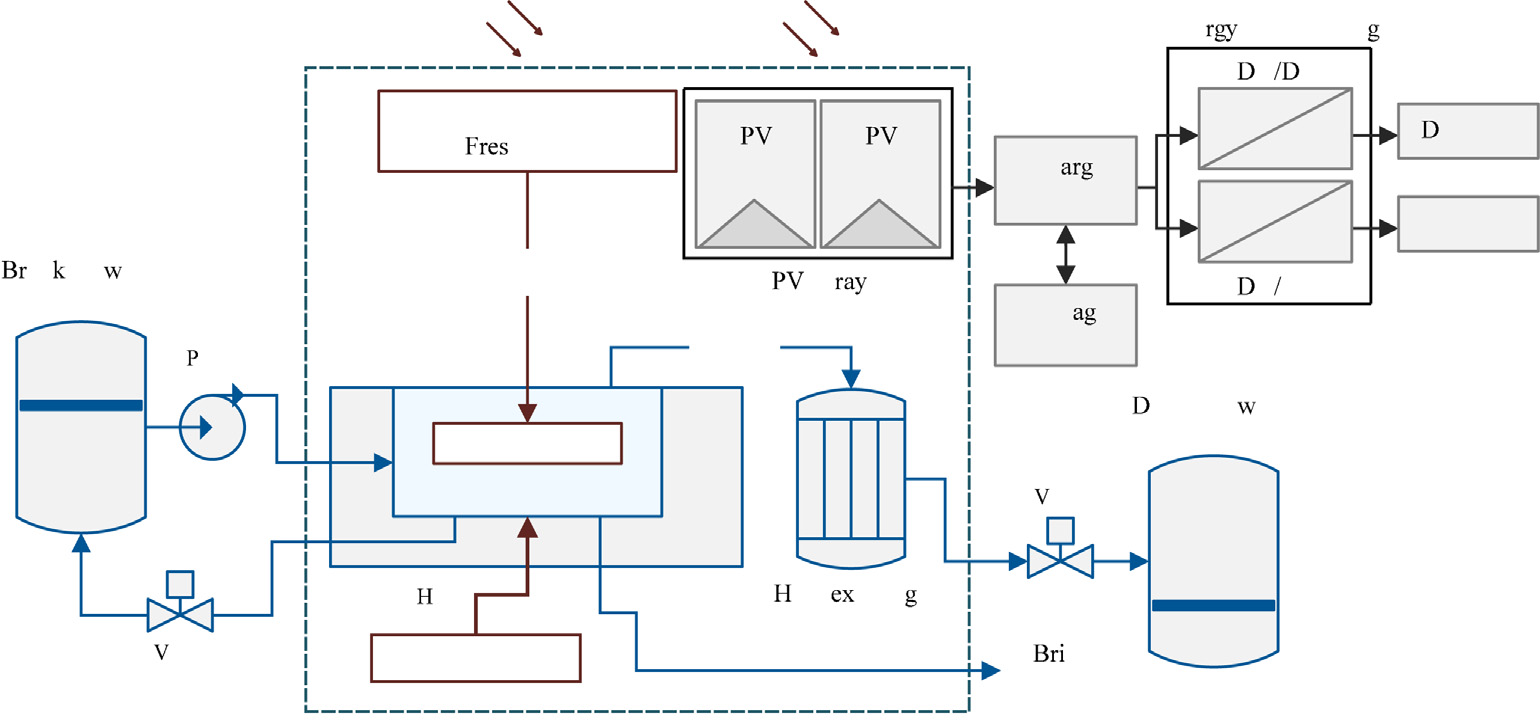
\includegraphics[
			height=45mm,
			width=\linewidth,
			keepaspectratio
		]{destilador-palomino.png}
		\caption{Destilador solar activo de Palomino et. al}
		{\scriptsize\fullcite{palomino-resendiz_design_2018}}
	\end{figure}
\end{frame}


\begin{frame}
	\frametitle{Desalinizador de doble cámara}
	En 2022 se desarrolló un destilador solar activo el cual tuvo una producción de \qty{4.03}{\litre\per\metre\tothe{2}} por día.\\
	\begin{figure}
		\centering
		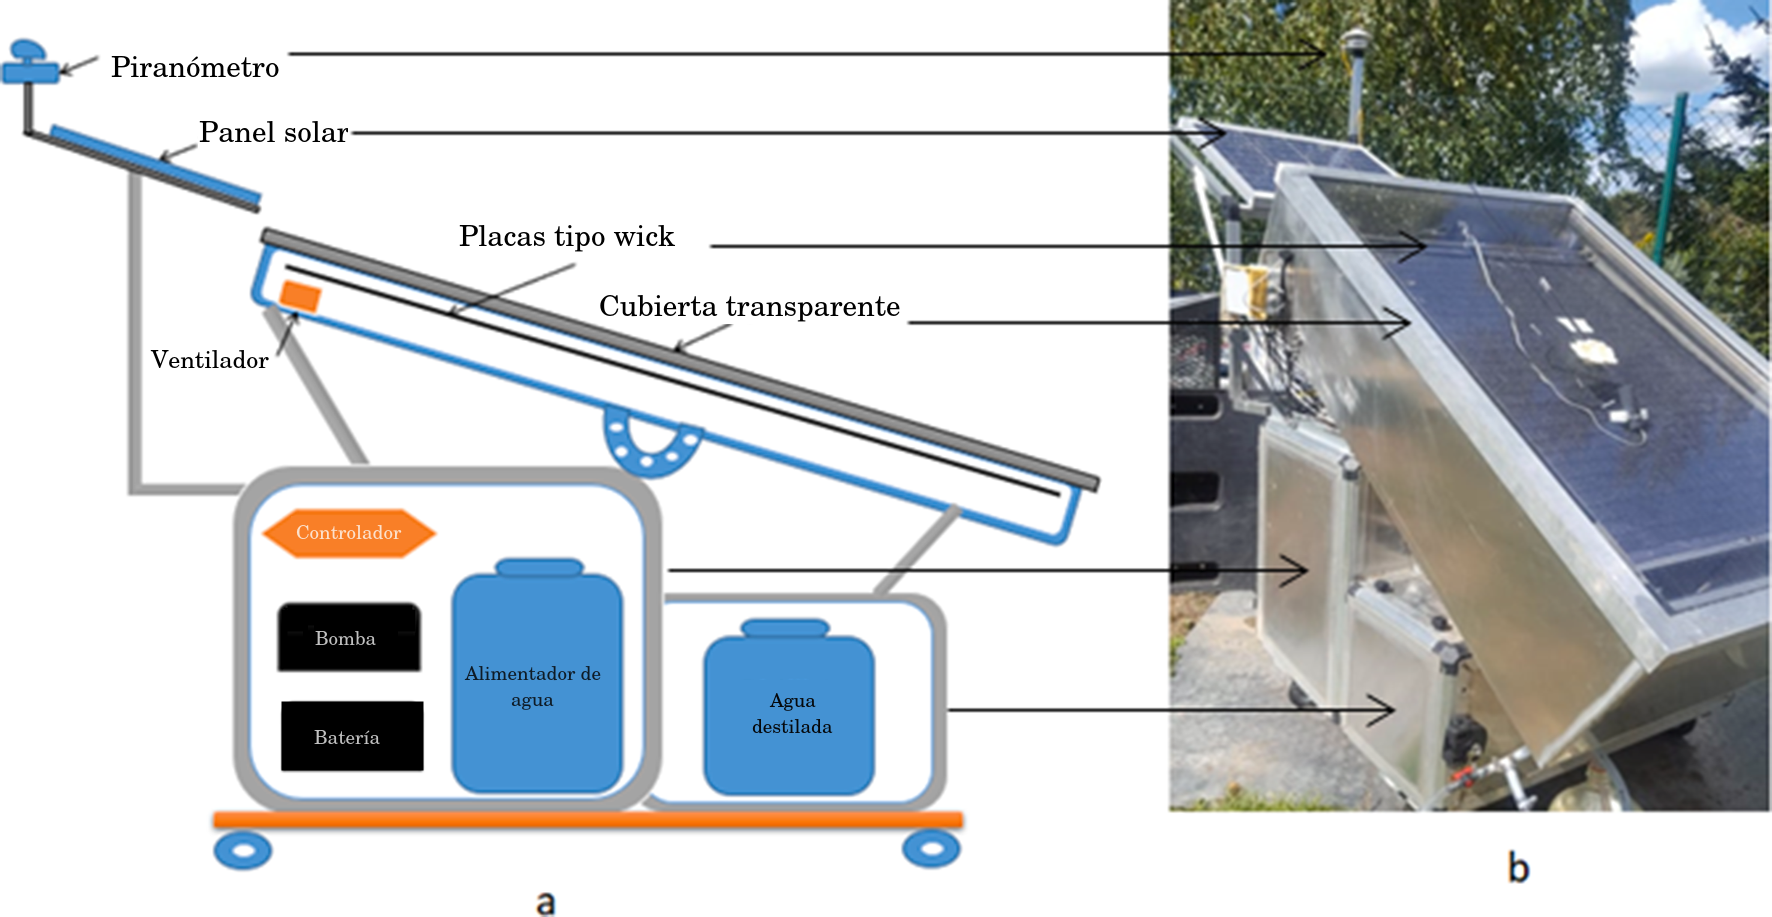
\includegraphics[
			height=45mm,
			width=\linewidth,
			keepaspectratio
		]{solar-wick-distiller.png}
		\caption{Destilador solar de doble cámara}
		{\scriptsize\fullcite{jobrane_theoretical_2022}}
	\end{figure}
\end{frame}

\subsection{Problemas asociados a la destilación solar}
	\begin{frame}
	    \frametitle{Problemas asociados a la destilación solar}
	    \vspace*{2mm}
	    
	    \textbf{\large Problemas identificados}\\[5mm]
	    
	    \begin{columns}
	    		\begin{column}{0.5\linewidth}
	    			\begin{figure}
	    				\includegraphics[
		    				width=\linewidth
	    				]{Desarrollo/condensación.jpg}
	    				\caption{Transmitancia afectada por la evaporación y la condensación}
	    			\end{figure}
		    \end{column}
		    \begin{column}{0.5\linewidth}
		    		\begin{figure}
	    				
\includegraphics[
		    				width=\linewidth
	    				]{Desarrollo/intermitencia.png}
	    				\caption{Forma de energía discontinua}
	    			\end{figure}
		    \end{column}
	    \end{columns}
	\end{frame}